% Options for packages loaded elsewhere
% Options for packages loaded elsewhere
\PassOptionsToPackage{unicode}{hyperref}
\PassOptionsToPackage{hyphens}{url}
\PassOptionsToPackage{dvipsnames,svgnames,x11names}{xcolor}
%
\documentclass[
  custompaper,
  DIV=11,
  numbers=noendperiod]{scrartcl}
\usepackage{xcolor}
\usepackage{amsmath,amssymb}
\setcounter{secnumdepth}{-\maxdimen} % remove section numbering
\usepackage{iftex}
\ifPDFTeX
  \usepackage[T1]{fontenc}
  \usepackage[utf8]{inputenc}
  \usepackage{textcomp} % provide euro and other symbols
\else % if luatex or xetex
  \usepackage{unicode-math} % this also loads fontspec
  \defaultfontfeatures{Scale=MatchLowercase}
  \defaultfontfeatures[\rmfamily]{Ligatures=TeX,Scale=1}
\fi
\usepackage{lmodern}
\ifPDFTeX\else
  % xetex/luatex font selection
\fi
% Use upquote if available, for straight quotes in verbatim environments
\IfFileExists{upquote.sty}{\usepackage{upquote}}{}
\IfFileExists{microtype.sty}{% use microtype if available
  \usepackage[]{microtype}
  \UseMicrotypeSet[protrusion]{basicmath} % disable protrusion for tt fonts
}{}
\makeatletter
\@ifundefined{KOMAClassName}{% if non-KOMA class
  \IfFileExists{parskip.sty}{%
    \usepackage{parskip}
  }{% else
    \setlength{\parindent}{0pt}
    \setlength{\parskip}{6pt plus 2pt minus 1pt}}
}{% if KOMA class
  \KOMAoptions{parskip=half}}
\makeatother
% Make \paragraph and \subparagraph free-standing
\makeatletter
\ifx\paragraph\undefined\else
  \let\oldparagraph\paragraph
  \renewcommand{\paragraph}{
    \@ifstar
      \xxxParagraphStar
      \xxxParagraphNoStar
  }
  \newcommand{\xxxParagraphStar}[1]{\oldparagraph*{#1}\mbox{}}
  \newcommand{\xxxParagraphNoStar}[1]{\oldparagraph{#1}\mbox{}}
\fi
\ifx\subparagraph\undefined\else
  \let\oldsubparagraph\subparagraph
  \renewcommand{\subparagraph}{
    \@ifstar
      \xxxSubParagraphStar
      \xxxSubParagraphNoStar
  }
  \newcommand{\xxxSubParagraphStar}[1]{\oldsubparagraph*{#1}\mbox{}}
  \newcommand{\xxxSubParagraphNoStar}[1]{\oldsubparagraph{#1}\mbox{}}
\fi
\makeatother


\usepackage{longtable,booktabs,array}
\usepackage{calc} % for calculating minipage widths
% Correct order of tables after \paragraph or \subparagraph
\usepackage{etoolbox}
\makeatletter
\patchcmd\longtable{\par}{\if@noskipsec\mbox{}\fi\par}{}{}
\makeatother
% Allow footnotes in longtable head/foot
\IfFileExists{footnotehyper.sty}{\usepackage{footnotehyper}}{\usepackage{footnote}}
\makesavenoteenv{longtable}
\usepackage{graphicx}
\makeatletter
\newsavebox\pandoc@box
\newcommand*\pandocbounded[1]{% scales image to fit in text height/width
  \sbox\pandoc@box{#1}%
  \Gscale@div\@tempa{\textheight}{\dimexpr\ht\pandoc@box+\dp\pandoc@box\relax}%
  \Gscale@div\@tempb{\linewidth}{\wd\pandoc@box}%
  \ifdim\@tempb\p@<\@tempa\p@\let\@tempa\@tempb\fi% select the smaller of both
  \ifdim\@tempa\p@<\p@\scalebox{\@tempa}{\usebox\pandoc@box}%
  \else\usebox{\pandoc@box}%
  \fi%
}
% Set default figure placement to htbp
\def\fps@figure{htbp}
\makeatother





\setlength{\emergencystretch}{3em} % prevent overfull lines

\providecommand{\tightlist}{%
  \setlength{\itemsep}{0pt}\setlength{\parskip}{0pt}}



 


\usepackage{fontawesome6}
\KOMAoption{captions}{tableheading}
\makeatletter
\@ifpackageloaded{tcolorbox}{}{\usepackage[skins,breakable]{tcolorbox}}
\@ifpackageloaded{fontawesome5}{}{\usepackage{fontawesome5}}
\definecolor{quarto-callout-color}{HTML}{909090}
\definecolor{quarto-callout-note-color}{HTML}{0758E5}
\definecolor{quarto-callout-important-color}{HTML}{CC1914}
\definecolor{quarto-callout-warning-color}{HTML}{EB9113}
\definecolor{quarto-callout-tip-color}{HTML}{00A047}
\definecolor{quarto-callout-caution-color}{HTML}{FC5300}
\definecolor{quarto-callout-color-frame}{HTML}{acacac}
\definecolor{quarto-callout-note-color-frame}{HTML}{4582ec}
\definecolor{quarto-callout-important-color-frame}{HTML}{d9534f}
\definecolor{quarto-callout-warning-color-frame}{HTML}{f0ad4e}
\definecolor{quarto-callout-tip-color-frame}{HTML}{02b875}
\definecolor{quarto-callout-caution-color-frame}{HTML}{fd7e14}
\makeatother
\makeatletter
\@ifpackageloaded{caption}{}{\usepackage{caption}}
\AtBeginDocument{%
\ifdefined\contentsname
  \renewcommand*\contentsname{Table of contents}
\else
  \newcommand\contentsname{Table of contents}
\fi
\ifdefined\listfigurename
  \renewcommand*\listfigurename{List of Figures}
\else
  \newcommand\listfigurename{List of Figures}
\fi
\ifdefined\listtablename
  \renewcommand*\listtablename{List of Tables}
\else
  \newcommand\listtablename{List of Tables}
\fi
\ifdefined\figurename
  \renewcommand*\figurename{Figure}
\else
  \newcommand\figurename{Figure}
\fi
\ifdefined\tablename
  \renewcommand*\tablename{Table}
\else
  \newcommand\tablename{Table}
\fi
}
\@ifpackageloaded{float}{}{\usepackage{float}}
\floatstyle{ruled}
\@ifundefined{c@chapter}{\newfloat{codelisting}{h}{lop}}{\newfloat{codelisting}{h}{lop}[chapter]}
\floatname{codelisting}{Listing}
\newcommand*\listoflistings{\listof{codelisting}{List of Listings}}
\makeatother
\makeatletter
\makeatother
\makeatletter
\@ifpackageloaded{caption}{}{\usepackage{caption}}
\@ifpackageloaded{subcaption}{}{\usepackage{subcaption}}
\makeatother
\makeatletter
\@ifpackageloaded{fontawesome6}{}{\usepackage{fontawesome6}}
\makeatother
\usepackage{bookmark}
\IfFileExists{xurl.sty}{\usepackage{xurl}}{} % add URL line breaks if available
\urlstyle{same}
\hypersetup{
  pdftitle={Quantitative Methoden mit R \& R-Studio},
  pdfauthor={Maura Kratz},
  colorlinks=true,
  linkcolor={blue},
  filecolor={Maroon},
  citecolor={Blue},
  urlcolor={Blue},
  pdfcreator={LaTeX via pandoc}}


\title{Quantitative Methoden mit R \& R-Studio}
\usepackage{etoolbox}
\makeatletter
\providecommand{\subtitle}[1]{% add subtitle to \maketitle
  \apptocmd{\@title}{\par {\large #1 \par}}{}{}
}
\makeatother
\subtitle{Sommersemester 2026 \textbar{} Sitzung 1}
\author{Maura Kratz}
\date{}
\begin{document}
\maketitle


\section{Was heute ansteht:}\label{was-heute-ansteht}

\begin{itemize}
\tightlist
\item
  Vorstellungsrunde
\item
  Warum computergestützte Datenanalyse lernen?
\item
  Warum R?
\item
  Was ist R? Was ist R-Studio?
\item
  Was erwartet uns in diesem Kurs?
\item
  Was ist bis kommenden Dienstag zu tun?
\end{itemize}

\section{Vorstellungsrunde}\label{vorstellungsrunde}

\subsection{Wer bin ich?}\label{wer-bin-ich}

übernehmen aus dem letzten kurs

\subsection{Wer seid ihr?}\label{wer-seid-ihr}

\section{Warum computergestützte Datenanalyse
lernen?}\label{warum-computergestuxfctzte-datenanalyse-lernen}

\subsection{Wir sind umgeben von
Daten}\label{wir-sind-umgeben-von-daten}

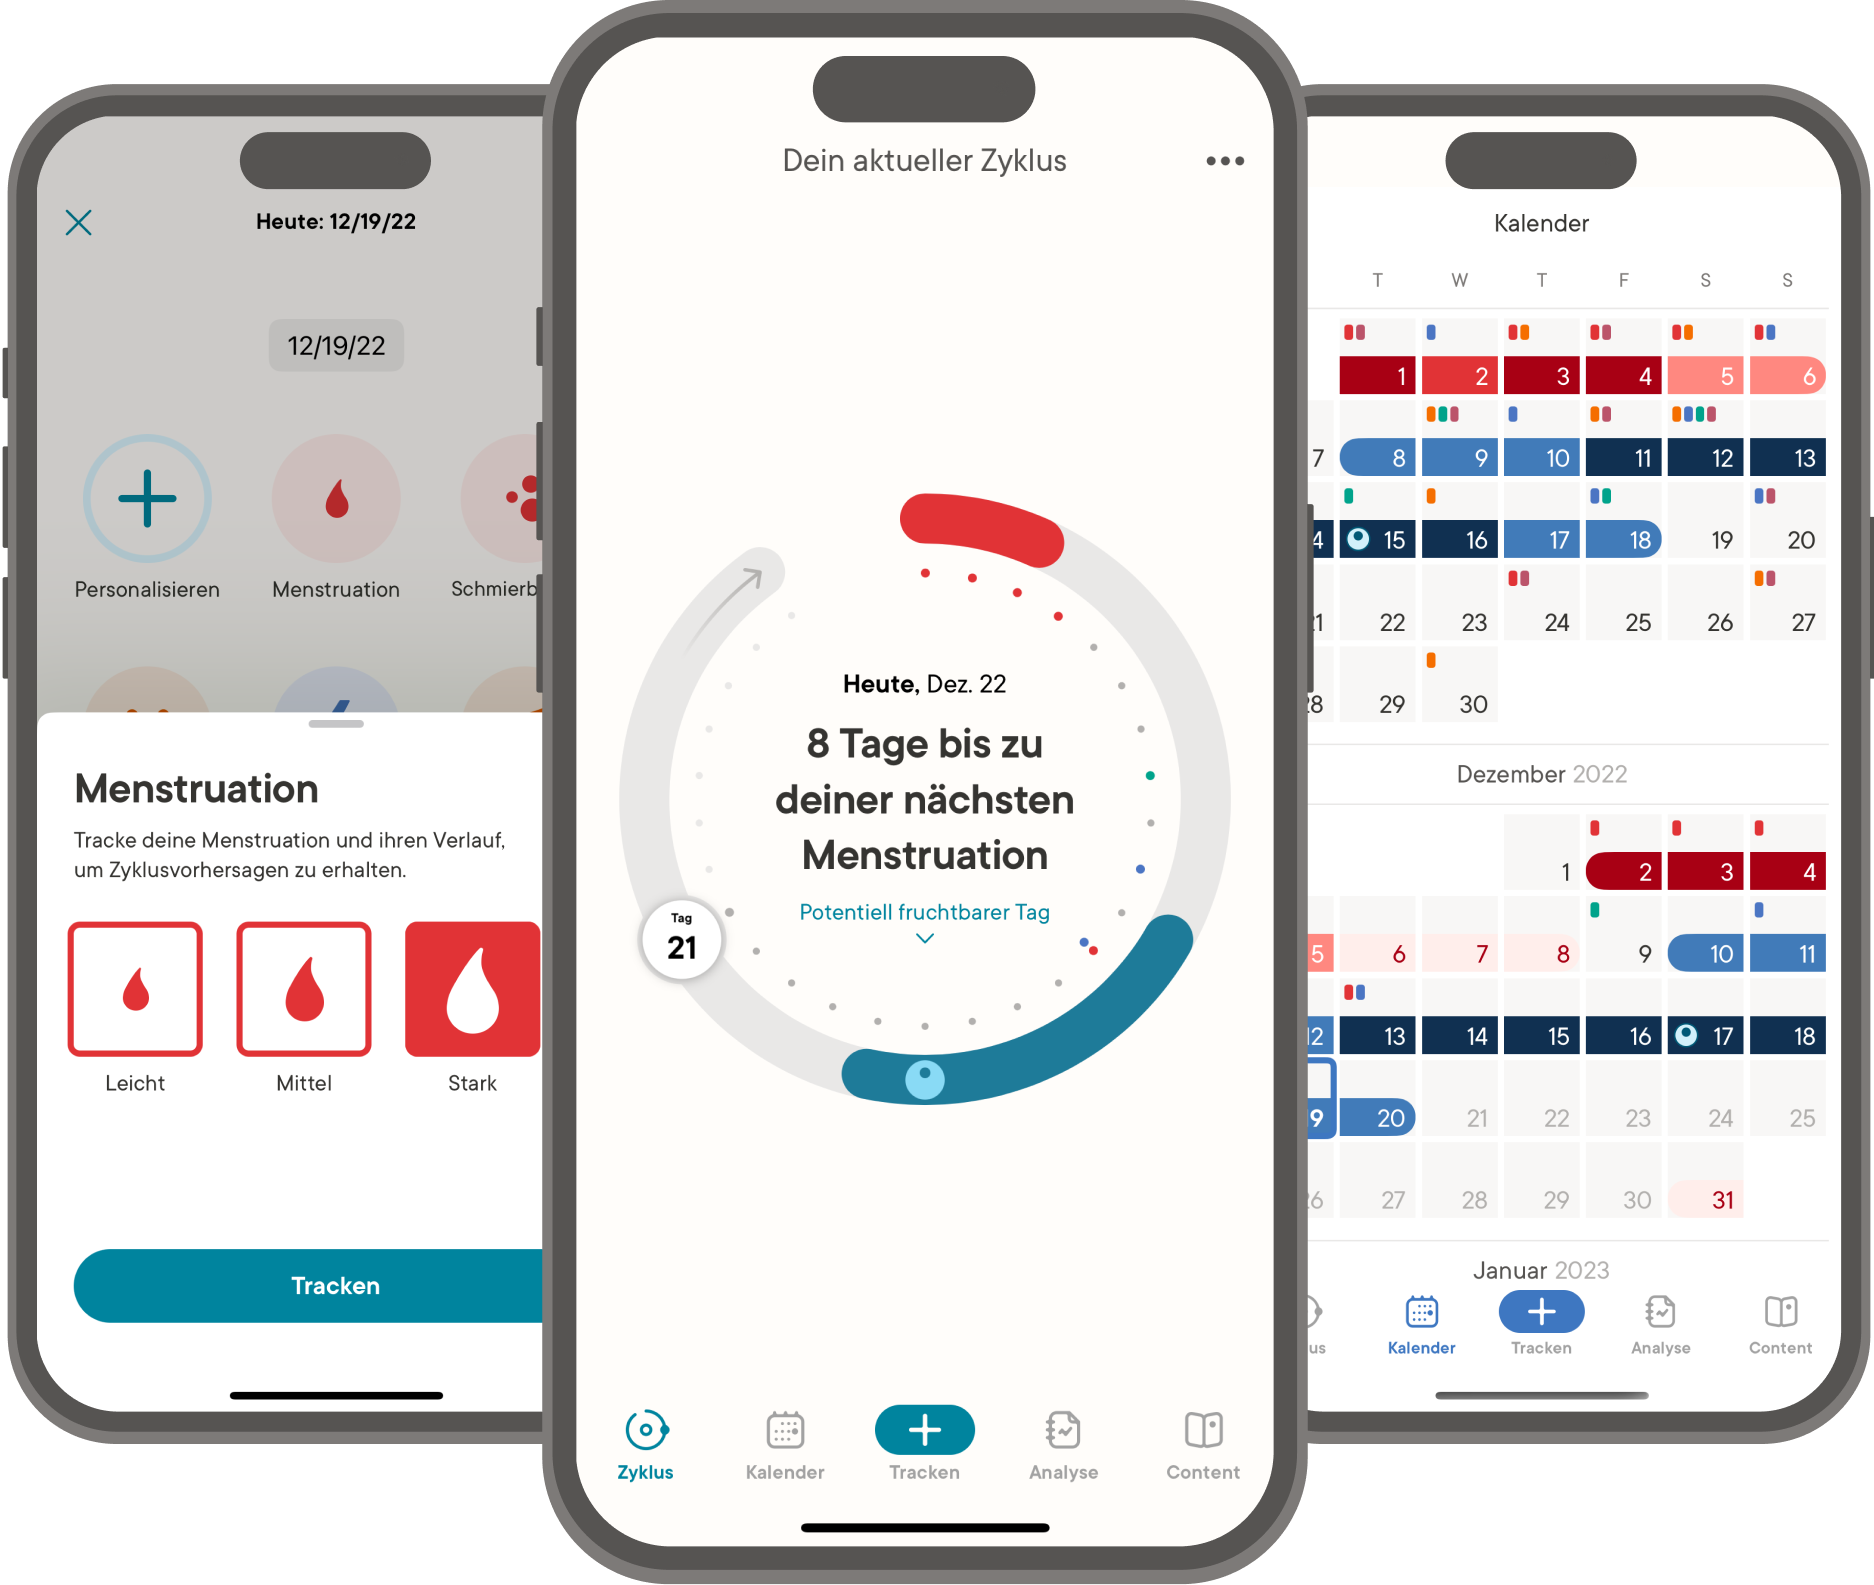
\includegraphics[width=0.8\linewidth,height=\textheight,keepaspectratio]{images/clipboard-4179089647.png}

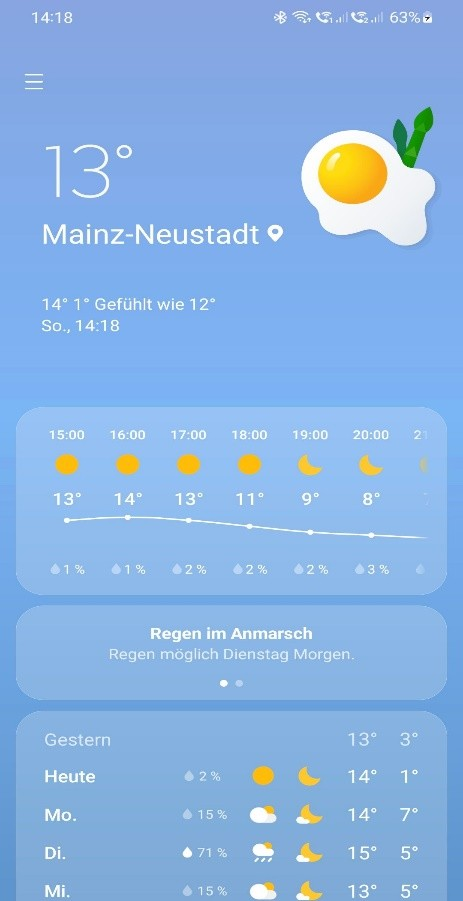
\includegraphics[width=0.8\linewidth,height=\textheight,keepaspectratio]{images/clipboard-361288377.jpeg}

\subsection{Daten helfen uns, soziale Phänomene zu
begreifen}\label{daten-helfen-uns-soziale-phuxe4nomene-zu-begreifen}

\pandocbounded{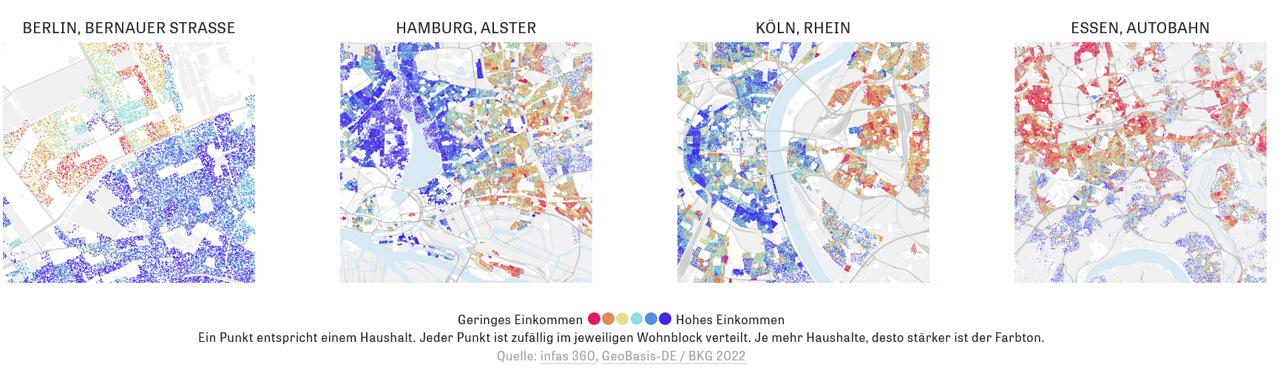
\includegraphics[keepaspectratio]{images/clipboard-1015560988.png}}

\subsection{Die Menge zu überblickender Daten wird immer
größer}\label{die-menge-zu-uxfcberblickender-daten-wird-immer-gruxf6uxdfer}

\begin{figure}

\begin{minipage}{0.50\linewidth}

\begin{figure}[H]

{\centering \pandocbounded{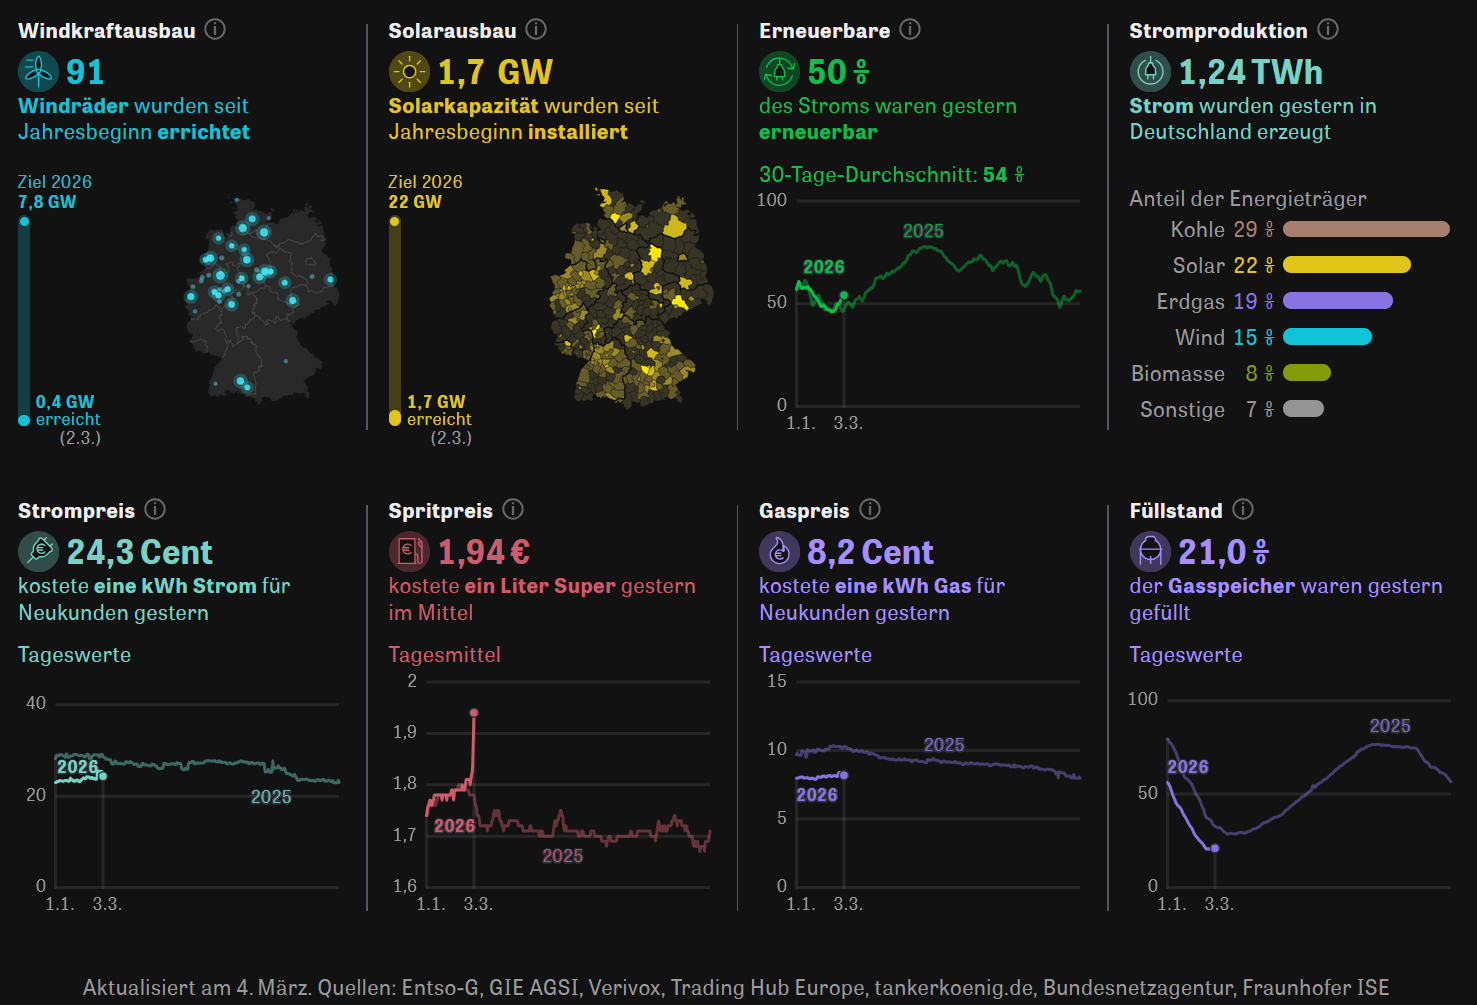
\includegraphics[keepaspectratio]{images/clipboard-2783348551.png}}

}

\subcaption{Quelle: Die Zeit.}

\end{figure}%

\end{minipage}%
%
\begin{minipage}{0.50\linewidth}
\pandocbounded{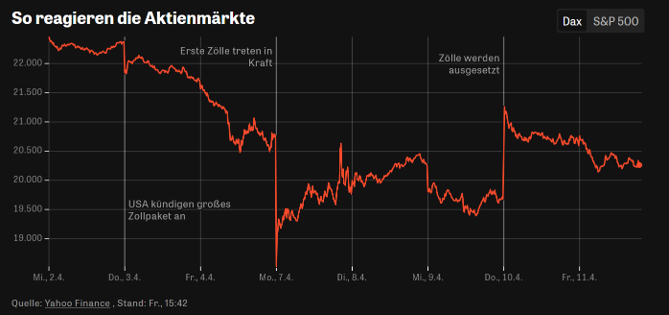
\includegraphics[keepaspectratio]{images/clipboard-185138689.png}}\end{minipage}%

\end{figure}%

\subsection{Datenkompetenz wird immer
wichtiger}\label{datenkompetenz-wird-immer-wichtiger}

\pandocbounded{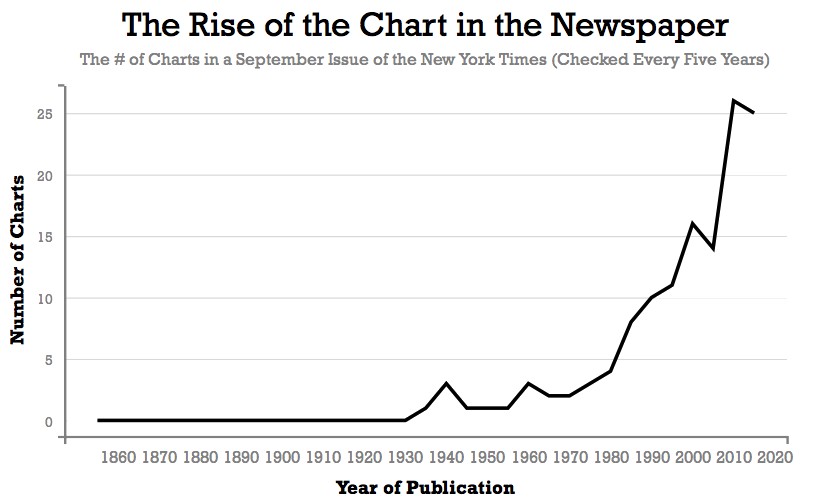
\includegraphics[keepaspectratio]{images/clipboard-2313191753.png}}

\subsection{Auch in der
Politikwissenschaft}\label{auch-in-der-politikwissenschaft}

\begin{figure}

\begin{minipage}{0.50\linewidth}
\pandocbounded{\includegraphics[keepaspectratio]{images/clipboard-2119200647.gif}}\end{minipage}%
%
\begin{minipage}{0.50\linewidth}
\pandocbounded{\includegraphics[keepaspectratio]{images/clipboard-4096817885.gif}}\end{minipage}%

\end{figure}%

Quelle: Monroe, Kristen Renwick, William Chiu, Adam Martin und Bridgette
Portman. 2009. What Is Political Psychology? Perspectives on Politics 7,
Nr. 4 (Dezember): 859--882. doi:10.1017/S153759270999185X.

\section{Aber warum ausgerechnet R für die computergestützte Datenanlyse
nutzen?}\label{aber-warum-ausgerechnet-r-fuxfcr-die-computergestuxfctzte-datenanlyse-nutzen}

\pandocbounded{
\includegraphics[keepaspectratio]{images/clipboard-4065168012.png}}

\subsection{Gängige
Statistik-Software}\label{guxe4ngige-statistik-software}

\pandocbounded{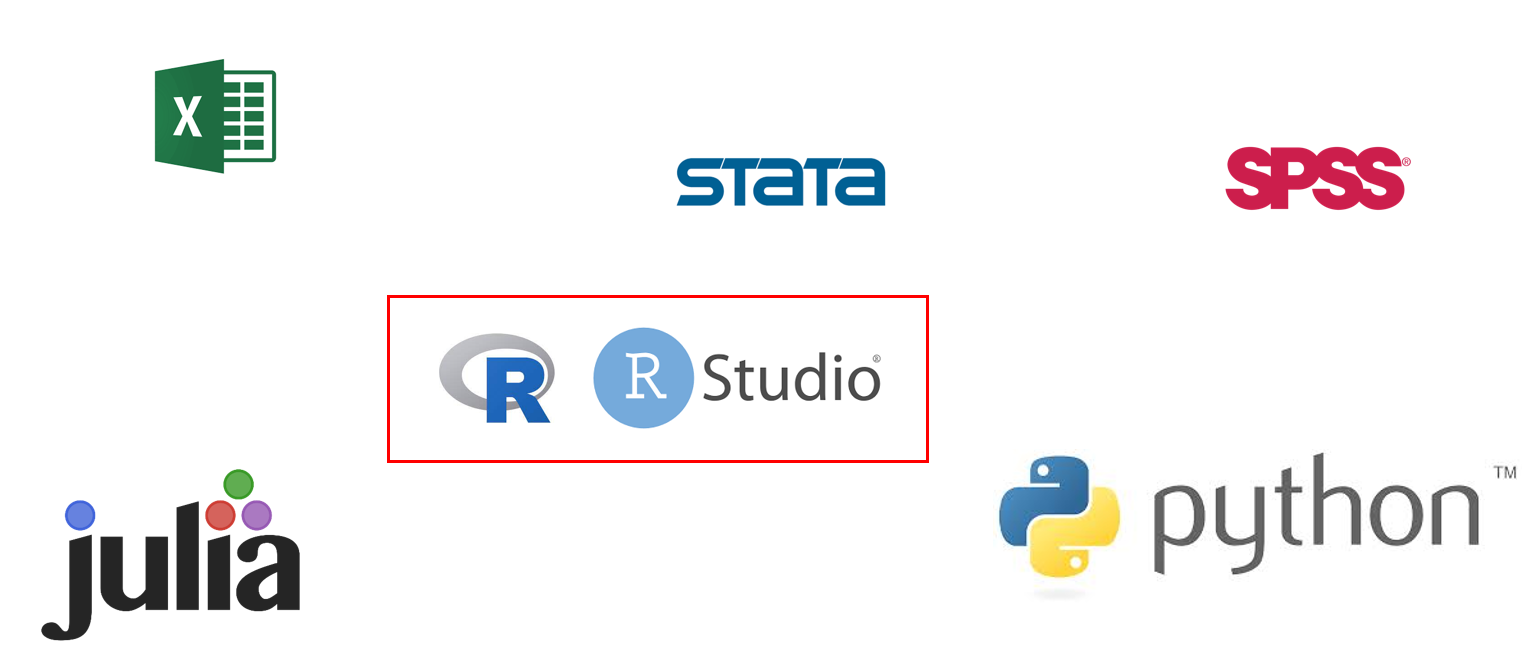
\includegraphics[keepaspectratio]{images/clipboard-1095058137.png}}

\subsection{}\label{section}

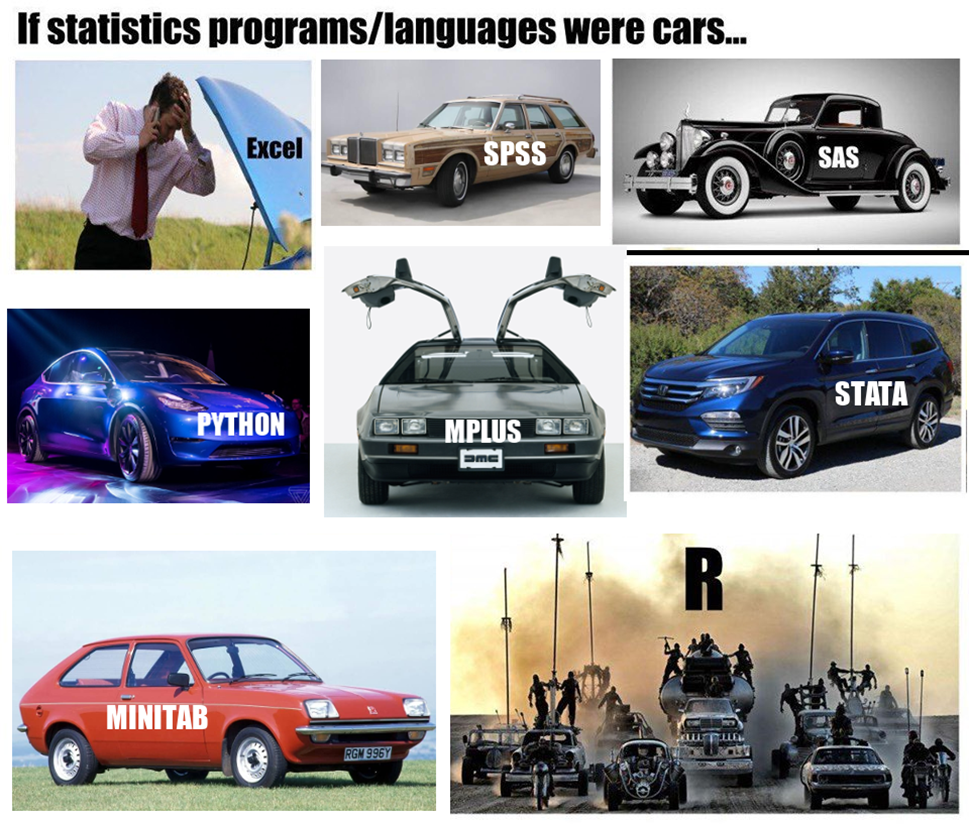
\includegraphics[width=0.6\linewidth,height=\textheight,keepaspectratio]{images/clipboard-3390527468.png}

\subsection{Warum R?}\label{warum-r}

\begin{itemize}
\tightlist
\item
  kostenlos \& für alle zugänglich \faIcon{thumbs-up}
\item
  kann (fast) alles → flexibel erweiterbar mit Paketen
  \faIcon{thumbs-up}
\item
  reproduzierbar \& transparent durch R-Skripte \faIcon{thumbs-up}
\item
  gut in andere Programme integrierbar \faIcon{thumbs-up}
\item
  versionierbar durch Gut und GitHub \faIcon{thumbs-up}
\item
  open-source → große Community \faIcon{thumbs-up}
\item
  Programmierkenntnisse erforderlich, daher weniger
  nutzer*innenfreundlich \faIcon{thumbs-down}
\end{itemize}

\subsection{R-Kenntnisse sind gefragt}\label{r-kenntnisse-sind-gefragt}

\begin{itemize}
\tightlist
\item
  klassische Berufsfelder für PoWi-Absolvent*innen: politische
  INstitutionen, Beratung, Verwaltung, Medien, NGOs, Projektmanagement
  \ldots{}
\item
  sie alle haben gemein, dass die Bedeutung evidenzbasierter und
  Entscheidungen zunimmt
\item
  R und Python für komplexe Datenanalysen
\item
  Zeitalter der AI → Data Science, Computational Science und
  maschinelles Lernen
\end{itemize}

\pandocbounded{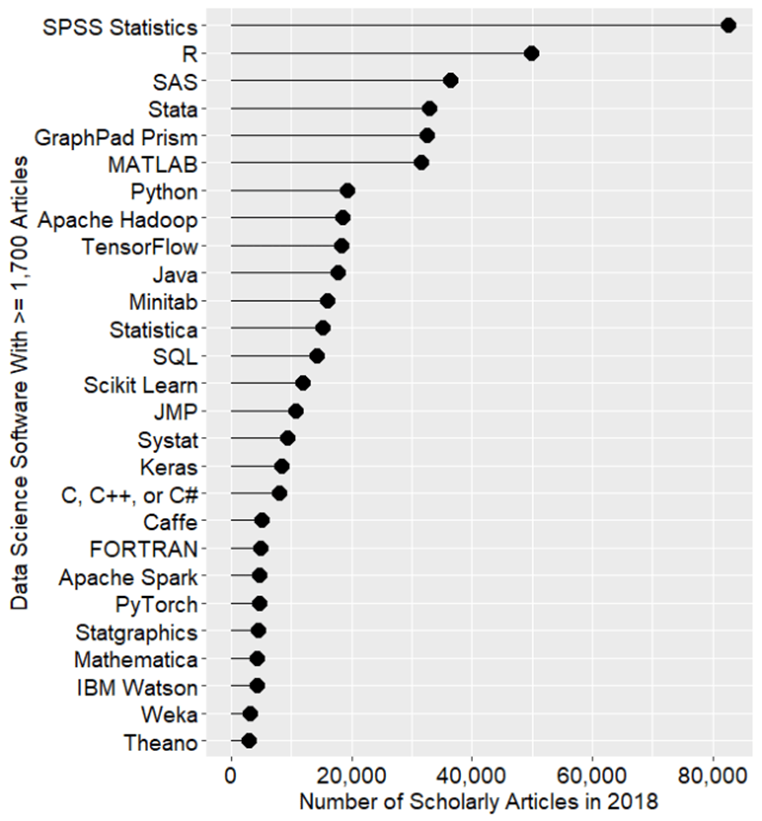
\includegraphics[keepaspectratio]{images/clipboard-492210661.png}}

\section{Was sind R und R-Studio
eigentlich?}\label{was-sind-r-und-r-studio-eigentlich}

\subsection{Was sind R und R-Studio?}\label{was-sind-r-und-r-studio}

\begin{itemize}
\tightlist
\item
  R ist eine Skriptsprache ( = „einfache`` Programmiersprache)
\item
  Ein Skript ist eine Abfolge von Befehlen
\item
  RStudio ist eine „Integrierte Entwicklungsumgebung'' (integrated
  development environment,IDE) für die Programmiersprache R → eine
  Umgebung die das Arbeiten mit R erleichtert
\end{itemize}

\begin{figure}

\begin{minipage}{0.50\linewidth}

\includegraphics[width=0.3\linewidth,height=\textheight,keepaspectratio]{images/clipboard-2230146645.png}

\includegraphics[width=0.5\linewidth,height=\textheight,keepaspectratio]{images/clipboard-3208056066.png}\end{minipage}%

\end{figure}%

\subsection{Was sind R und R-Studio?}\label{was-sind-r-und-r-studio-1}

\pandocbounded{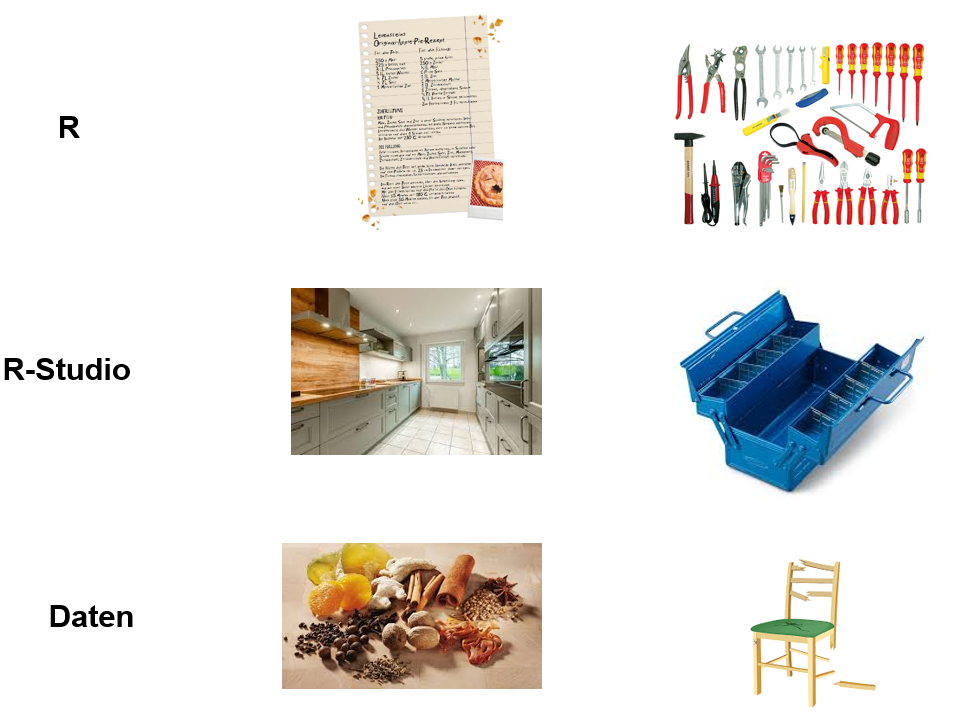
\includegraphics[keepaspectratio]{images/clipboard-4253454986.png}}

\subsection{Was sind R und R-Studio?}\label{was-sind-r-und-r-studio-2}

\begin{figure}

\begin{minipage}{0.50\linewidth}

\begin{figure}[H]

{\centering \pandocbounded{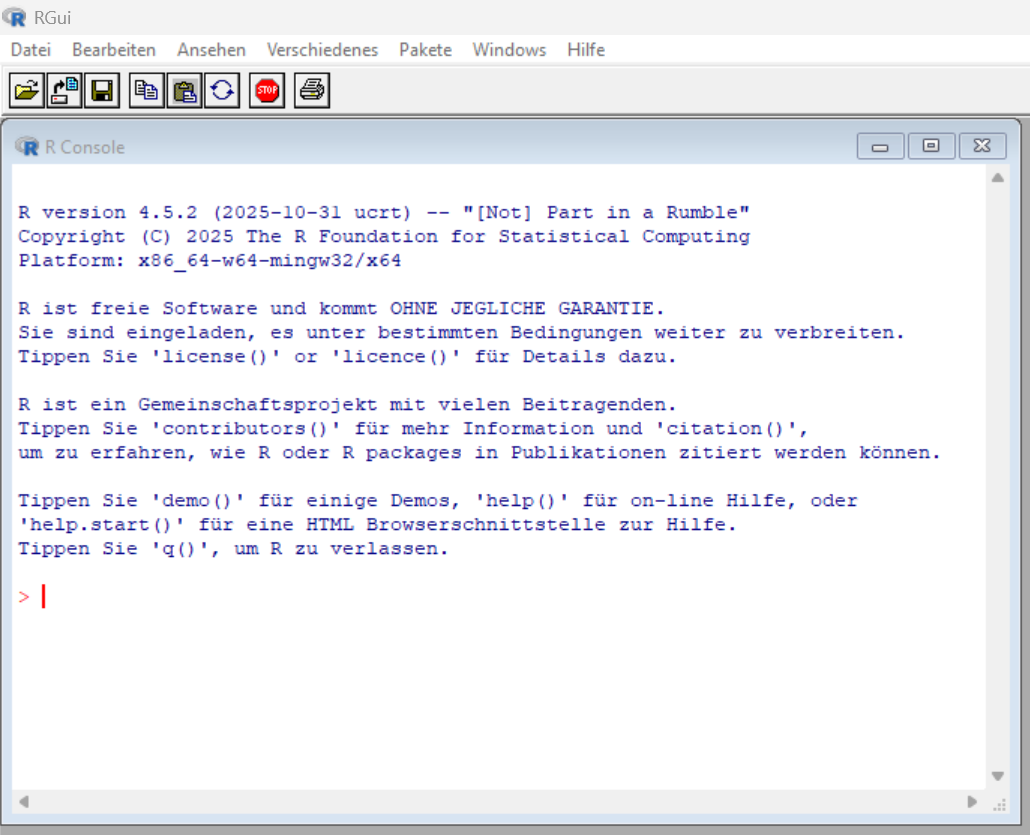
\includegraphics[keepaspectratio]{images/clipboard-825709011.png}}

}

\subcaption{R ohne R-Studio (in R-Gui)}

\end{figure}%

\end{minipage}%
%
\begin{minipage}{0.50\linewidth}

\begin{figure}[H]

{\centering \pandocbounded{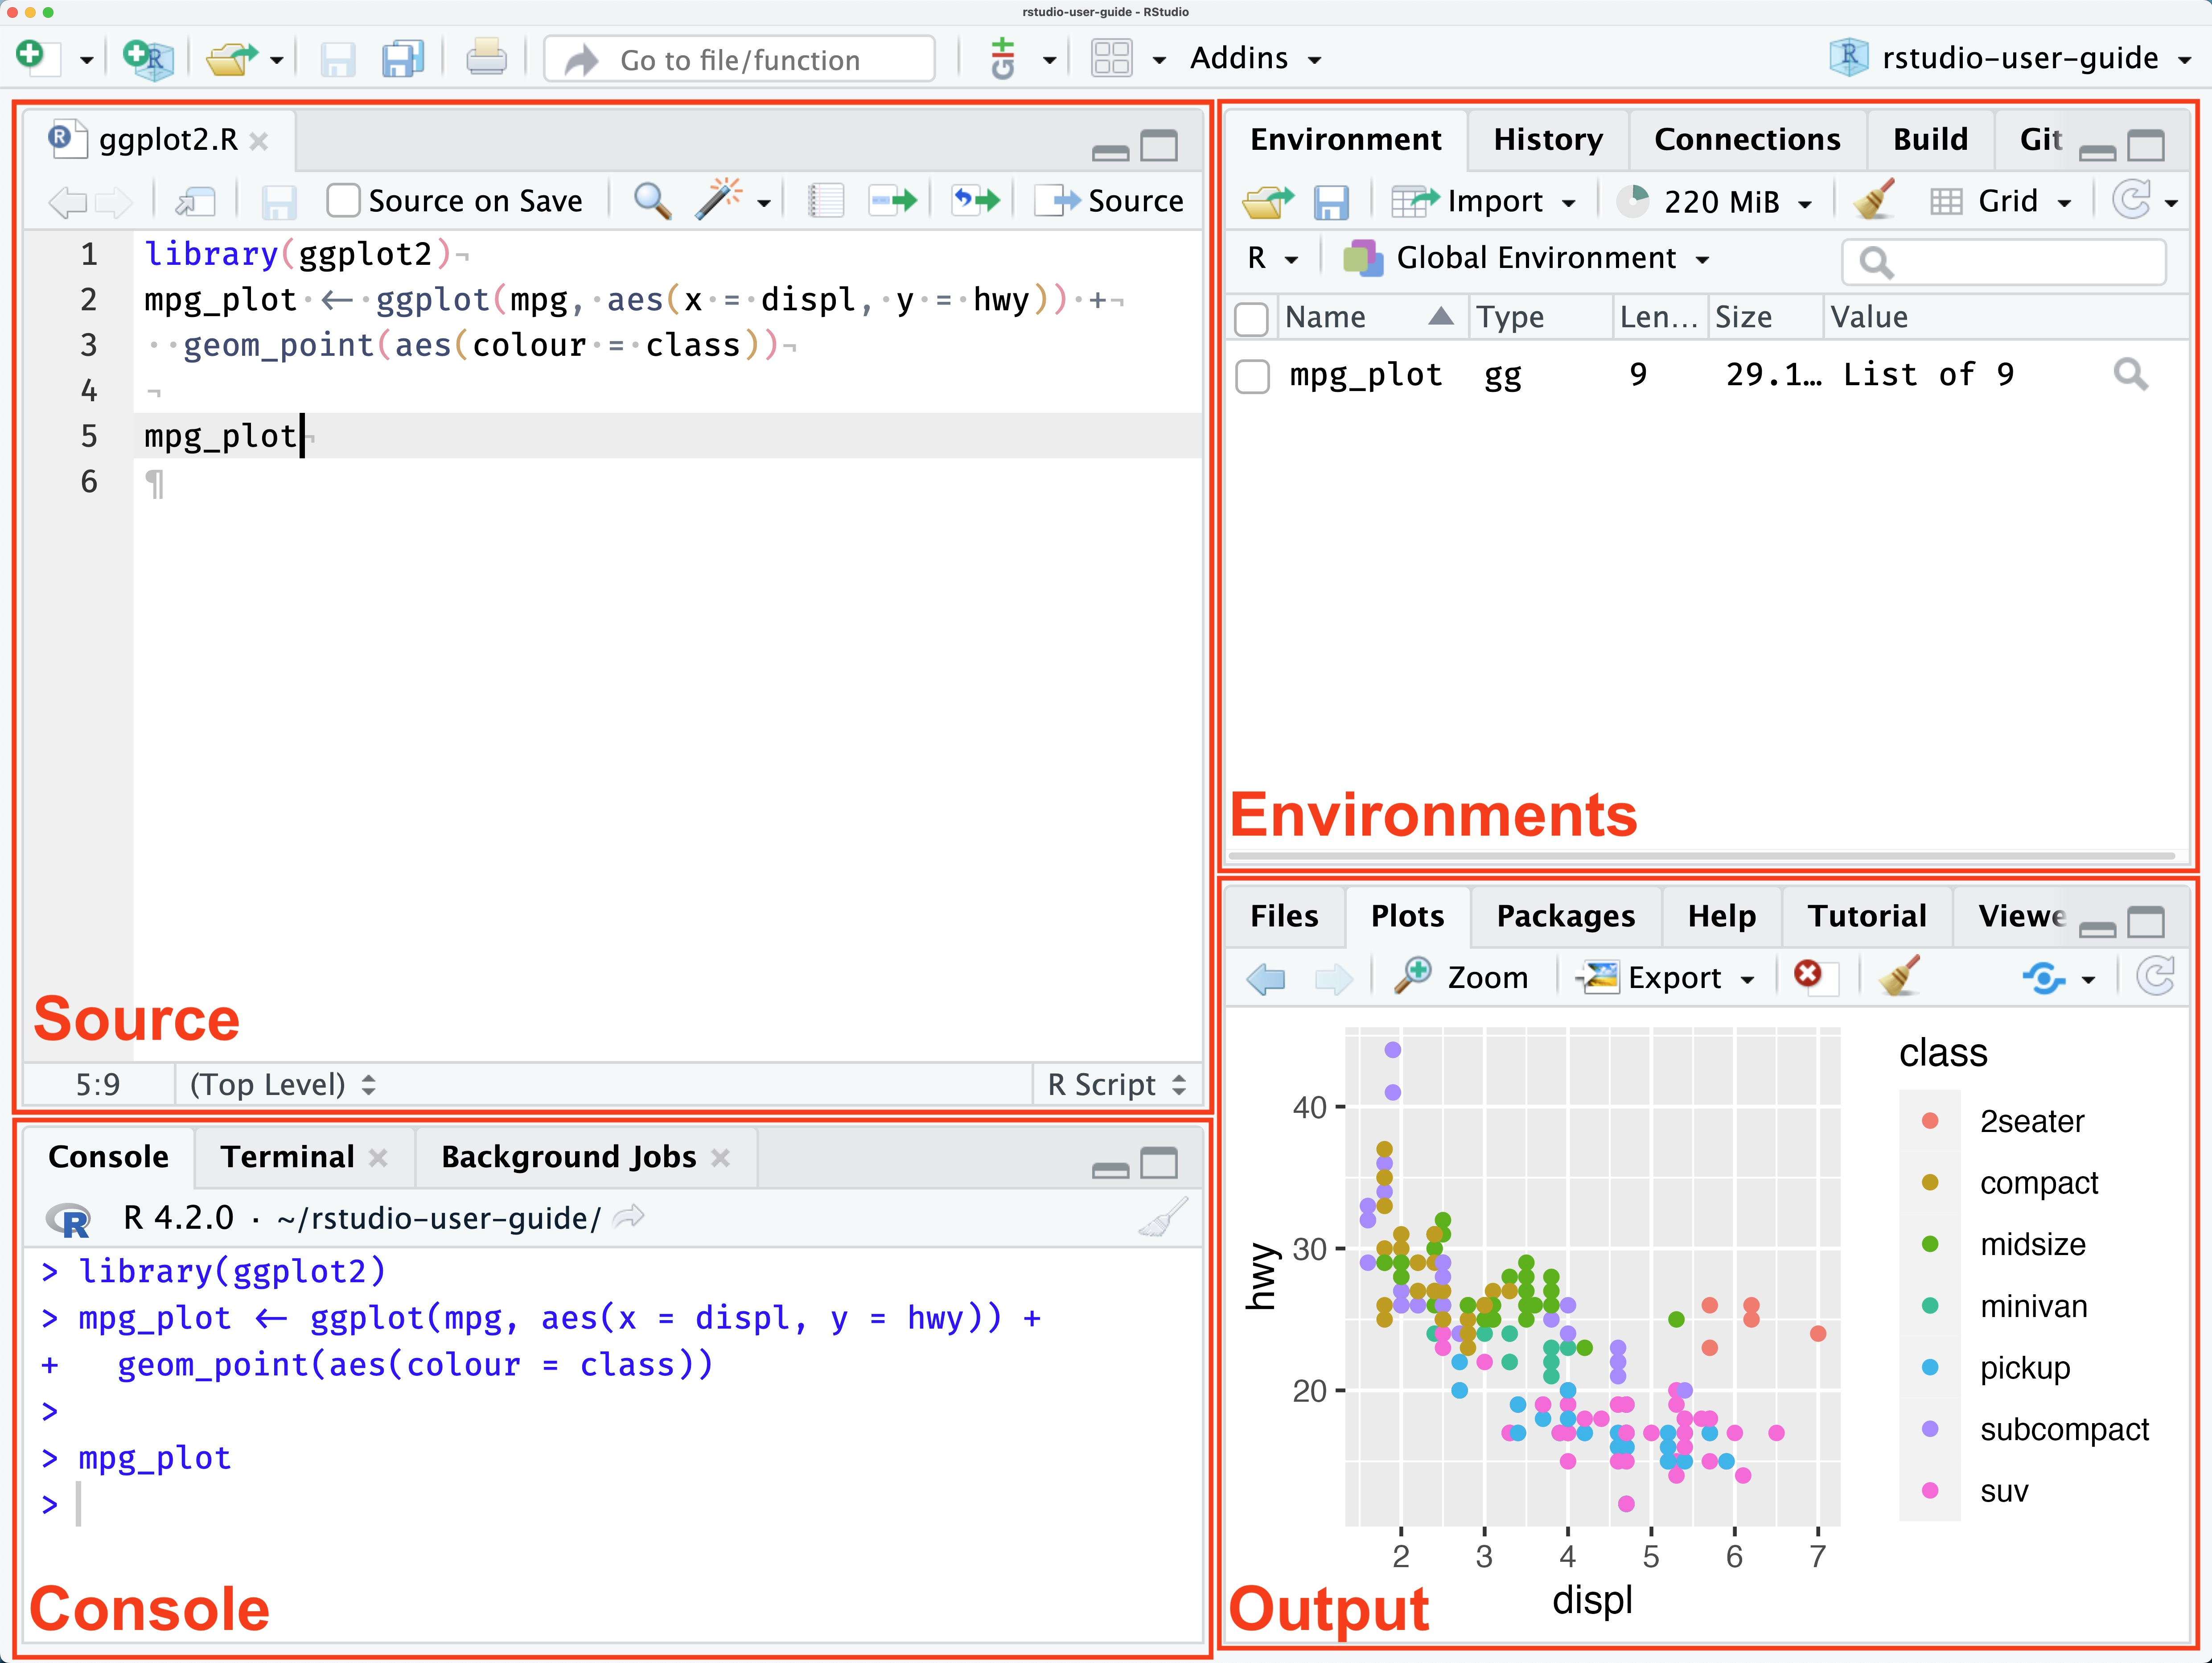
\includegraphics[keepaspectratio]{images/clipboard-3138135745.png}}

}

\subcaption{R in R-Studio}

\end{figure}%

\end{minipage}%

\end{figure}%

\subsection{Die goldenen R-Regeln}\label{die-goldenen-r-regeln}

\begin{figure}

\begin{minipage}{0.50\linewidth}

\begin{itemize}
\tightlist
\item
  Es gibt IMMER mehr als einen Weg zum Ziel
\item
  Gerade zu Beginn kann das Programmieren sehr frustrierend sein.
\item
  Gib nicht auf! Frustrationstoleranz ist der Schlüssel!
\end{itemize}

\end{minipage}%
%
\begin{minipage}{0.50\linewidth}
\pandocbounded{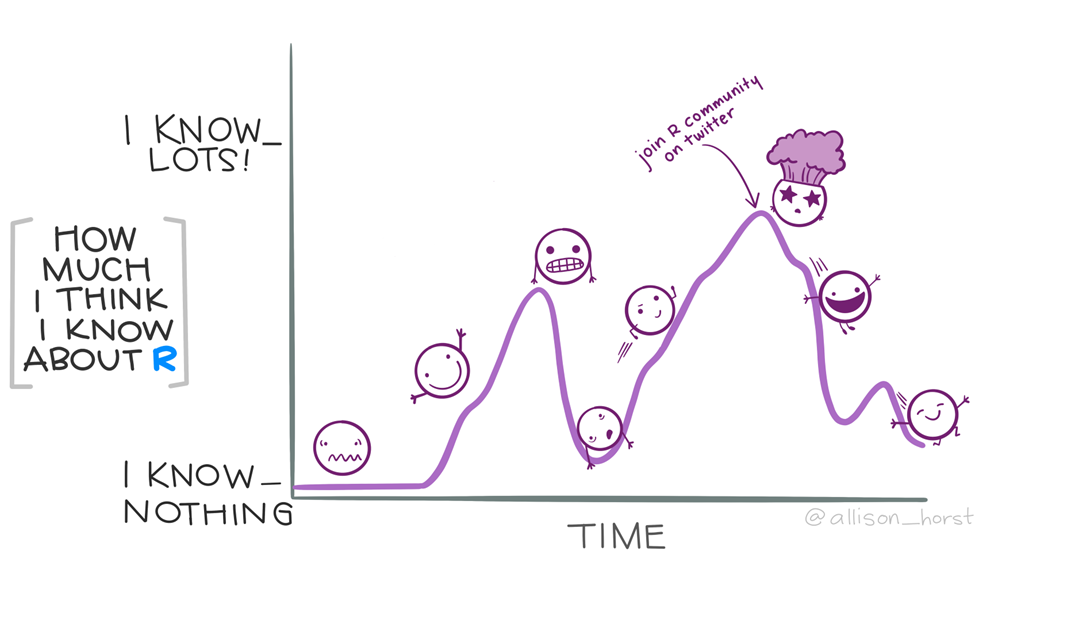
\includegraphics[keepaspectratio]{images/clipboard-989640835.png}}\end{minipage}%

\end{figure}%

\subsection{Datenanalyse-Workflow}\label{datenanalyse-workflow}

\begin{figure}

\begin{minipage}{0.50\linewidth}

\begin{enumerate}
\def\labelenumi{\arabic{enumi}.}
\tightlist
\item
  data import
\item
  data wrangling → data cleaning \& data transformation
\item
  overview → descriptives \& visualisation
\item
  modelling \& visualisation
\item
  interpreting the results
\end{enumerate}

\end{minipage}%
%
\begin{minipage}{0.50\linewidth}
\pandocbounded{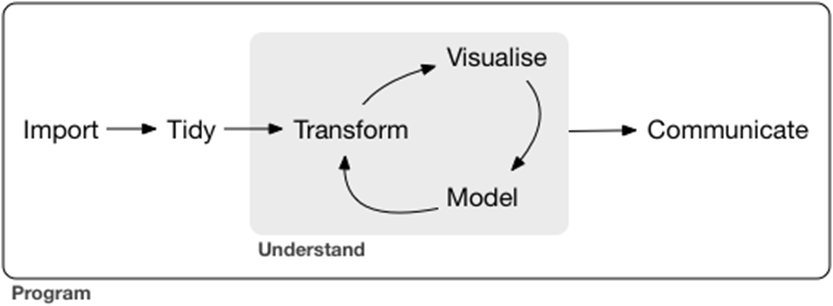
\includegraphics[keepaspectratio]{images/clipboard-1920433520.png}}\end{minipage}%

\end{figure}%

\subsection{Lernziel}\label{lernziel}

Erwerb der Fähigkeit, große Datensätze selbständig zu verarbeiten, den
Daten und der Fragestellung entsprechende geeignete Analysen
durchzuführen und deren Ergebnisse kompetent darzustellen und zu
interpretieren.

\subsection{Dieser Kurs vermittelt:}\label{dieser-kurs-vermittelt}

\begin{itemize}
\tightlist
\item
  Praktische Anwendung durch Übungen
\item
  Erlernen von Datenaufbereitung (Bereinigung und Bearbeitung),
\item
  Deskriptiver Datenanalyse,
\item
  Erster statistischer Datenanalyse und
\item
  Visualisierung und Darstellung
\end{itemize}

→ Übertragung auf kommende Lehrveranstaltungen, Hausarbeiten etc.

\subsection{Syllabus}\label{syllabus}

\begin{itemize}
\tightlist
\item
  Sitzungsplan
\item
  Zu erbringende Leistungen
\item
  Ressourcen
\item
  Tipps
\end{itemize}

\begin{tcolorbox}[enhanced jigsaw, arc=.35mm, titlerule=0mm, breakable, toprule=.15mm, opacityback=0, left=2mm, title=\textcolor{quarto-callout-important-color}{\faExclamation}\hspace{0.5em}{Wichtig}, colbacktitle=quarto-callout-important-color!10!white, opacitybacktitle=0.6, toptitle=1mm, bottomtitle=1mm, colframe=quarto-callout-important-color-frame, coltitle=black, rightrule=.15mm, bottomrule=.15mm, leftrule=.75mm, colback=white]

Der aktueller Syllabus sowie die Folien stehen auf Moodle/ GitHub zur
Verfügung.

\end{tcolorbox}

\subsection{Syllabus}\label{syllabus-1}

\pandocbounded{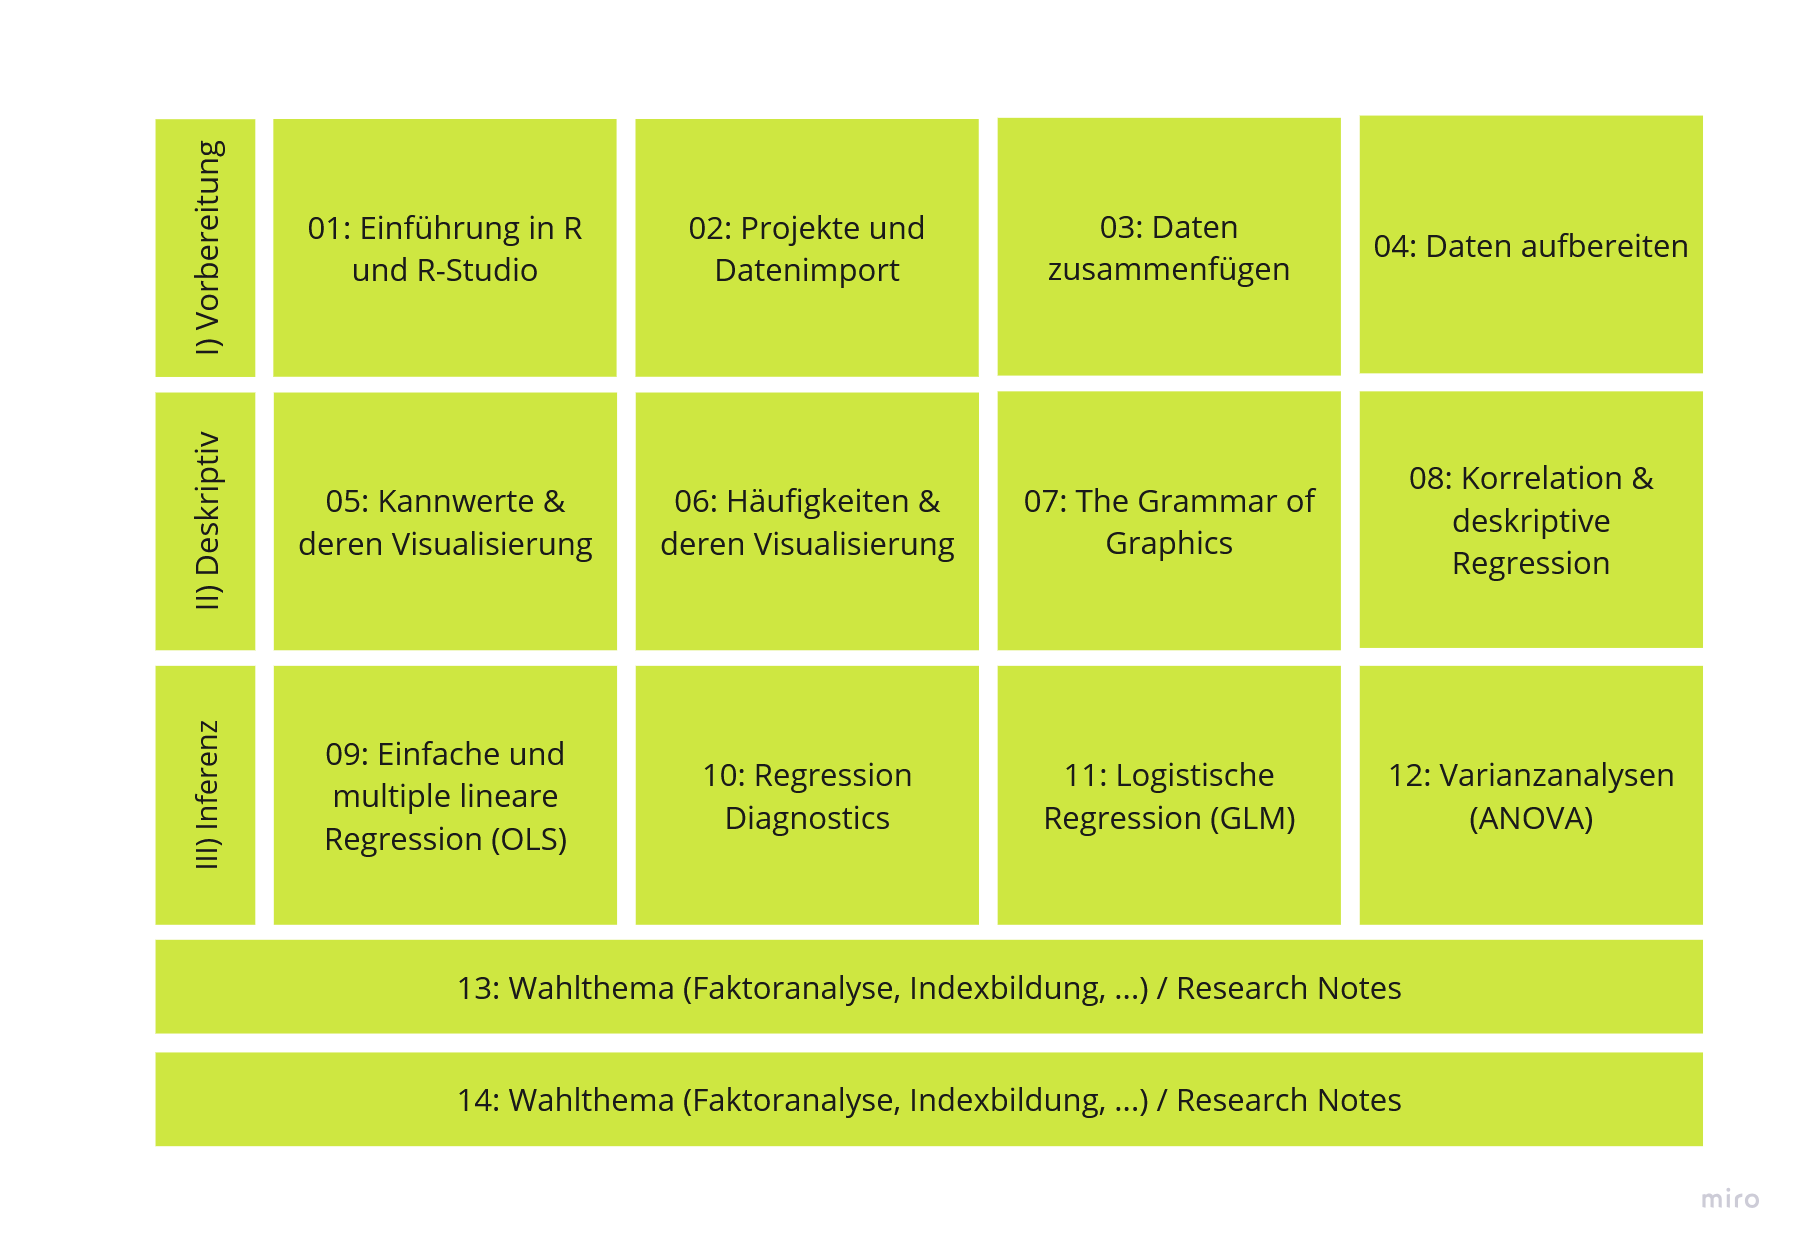
\includegraphics[keepaspectratio]{images/clipboard-1010800426.png}}

\subsection{Bis zur kommenden Sitzung
bitte}\label{bis-zur-kommenden-sitzung-bitte}

\begin{itemize}
\tightlist
\item
  R herunterladen \& installieren
\item
  R-Studio herunterladen \& installieren
\item
  mit dem Syllabus vertraut machen
\item
  etwaige Fragen notieren und zur nächsten Sitzung mitbringen
\end{itemize}

\subsection{R installieren}\label{r-installieren}

\begin{itemize}
\item
  Download über Website des Cran-Projekts („The Comprehensive R Archive
  Network``): \url{https://cran.uni-muenster.de/} oder
  \url{https://cloud.r-project.org/}

  \begin{itemize}
  \item
    Download and Install R → entsprechende Betriebssystem auswählen
    (Windows, Mac oder Linux)
  \item
    install R for the first time → aktuelle R-Version zum Download
    auswählen bzw. bei Mac entweder Mac mit mind. M1 Chip oder mit
    Intel-Prozessor auswählen
  \end{itemize}
\item
  Datei installieren (Standardeinstellungen können beibehalten werden)
\end{itemize}

\subsection{R installieren}\label{r-installieren-1}

\pandocbounded{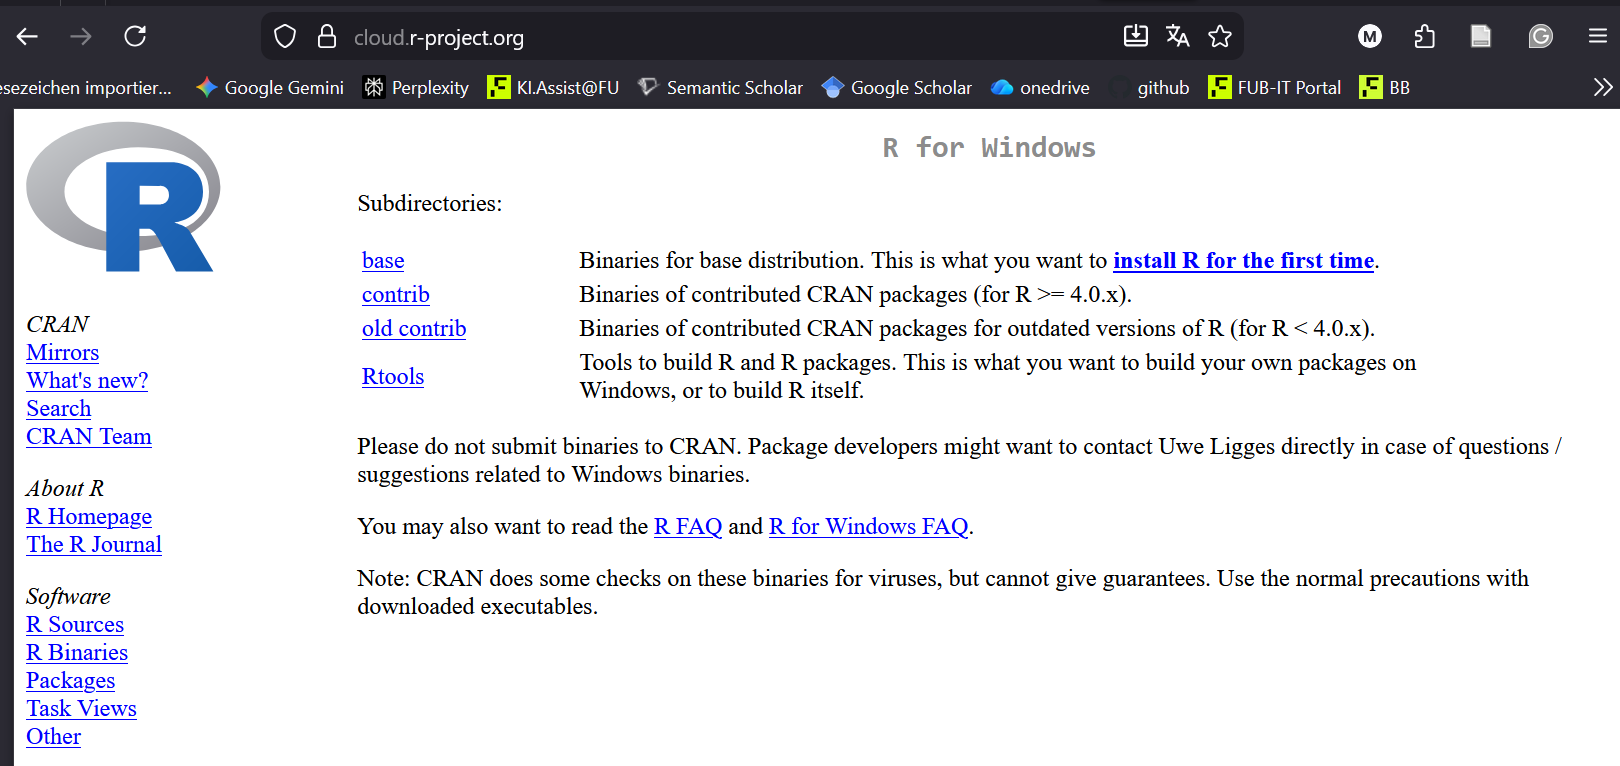
\includegraphics[keepaspectratio]{images/clipboard-3697793632.png}}

\pandocbounded{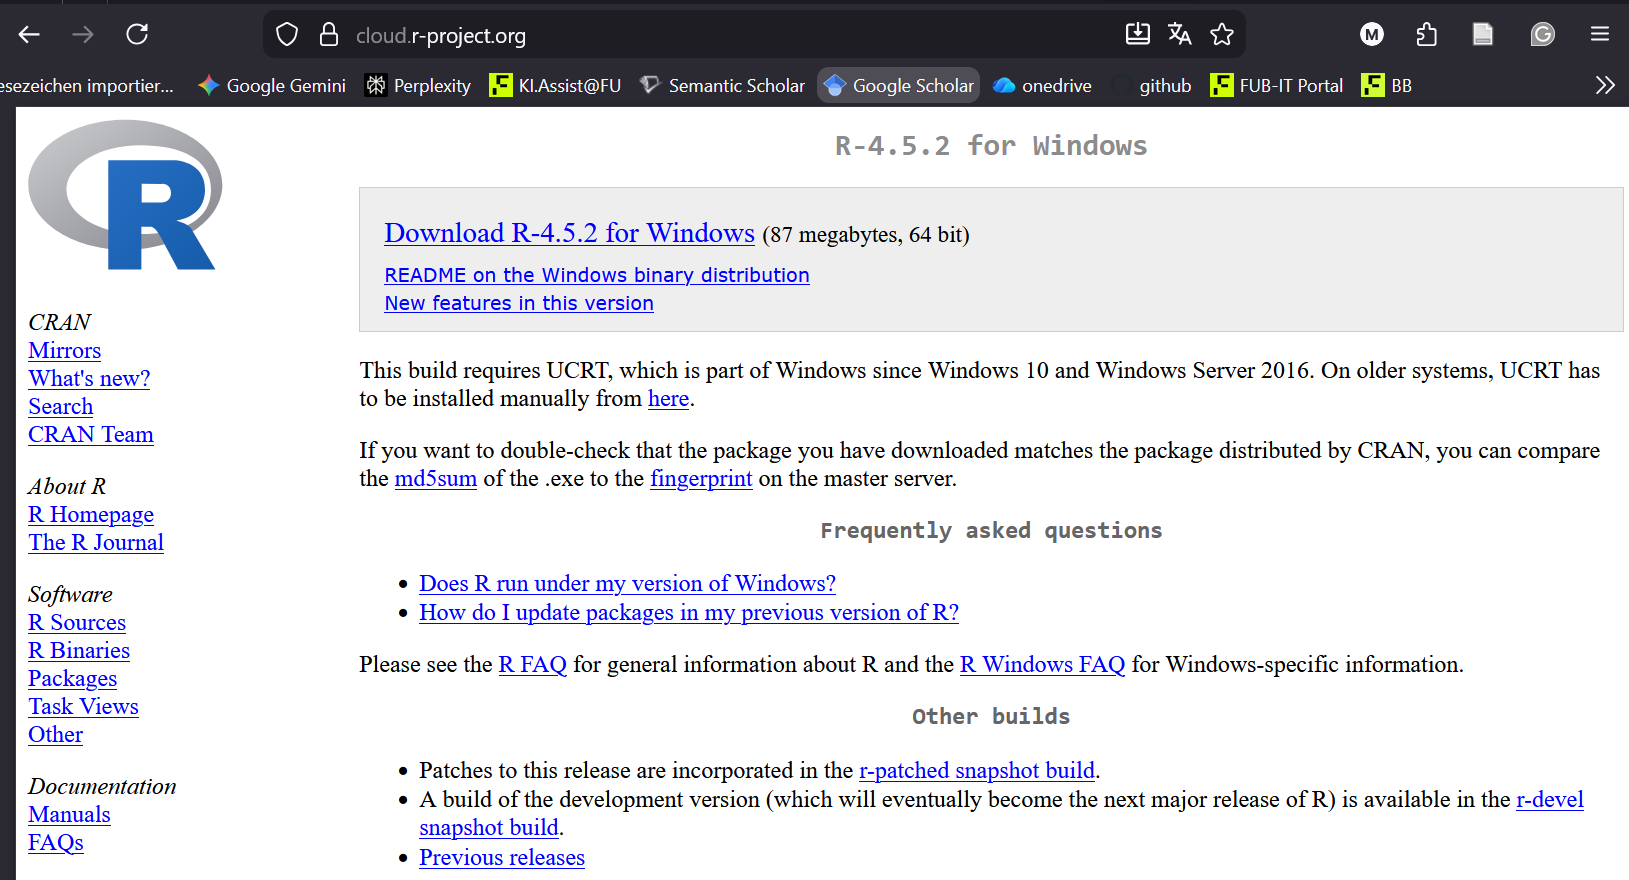
\includegraphics[keepaspectratio]{images/clipboard-2565061375.png}}

\pandocbounded{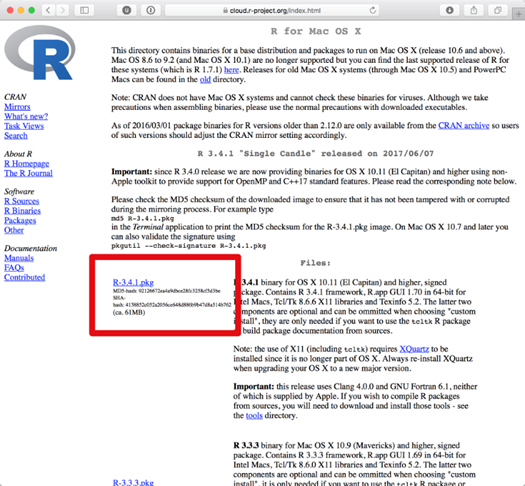
\includegraphics[keepaspectratio]{images/clipboard-2302214045.png}}

\subsection{R-Studio installieren}\label{r-studio-installieren}

\begin{itemize}
\tightlist
\item
  Download über Website von RStudio:
  \url{https://rstudio.com/products/rstudio/download/}
\item
  RStudio Desktop (Free-Lizenz und entsprechendes Betriebssystem)
  auswählen
\item
  Datei installieren
\item
  RStudio starten
\end{itemize}

\subsection{R-Studio installieren}\label{r-studio-installieren-1}

\pandocbounded{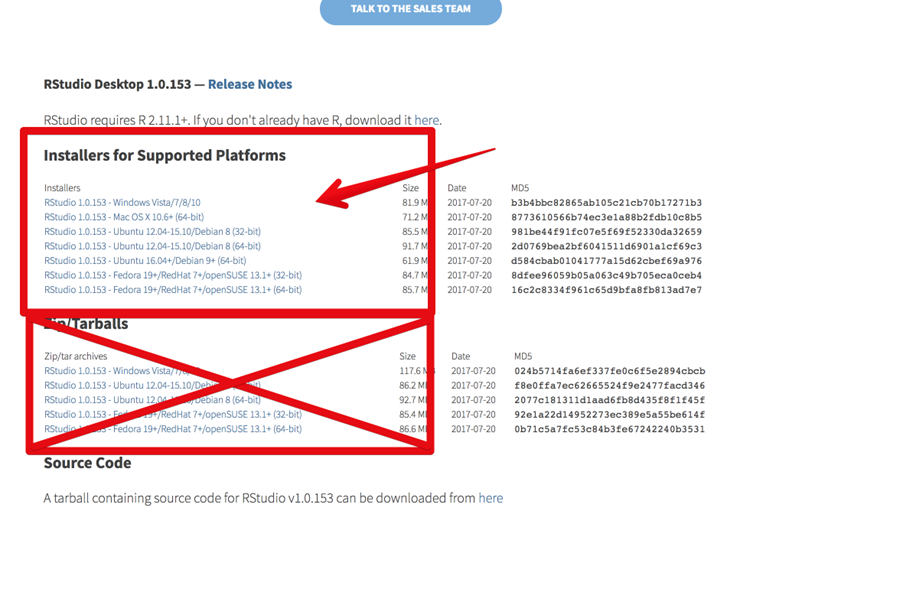
\includegraphics[keepaspectratio]{images/clipboard-1889837894.png}}

\subsection{R-Studio öffnen}\label{r-studio-uxf6ffnen}

Wenn du R-Studio das erste Mal öffnest, sieht es in etwa so aus:

\pandocbounded{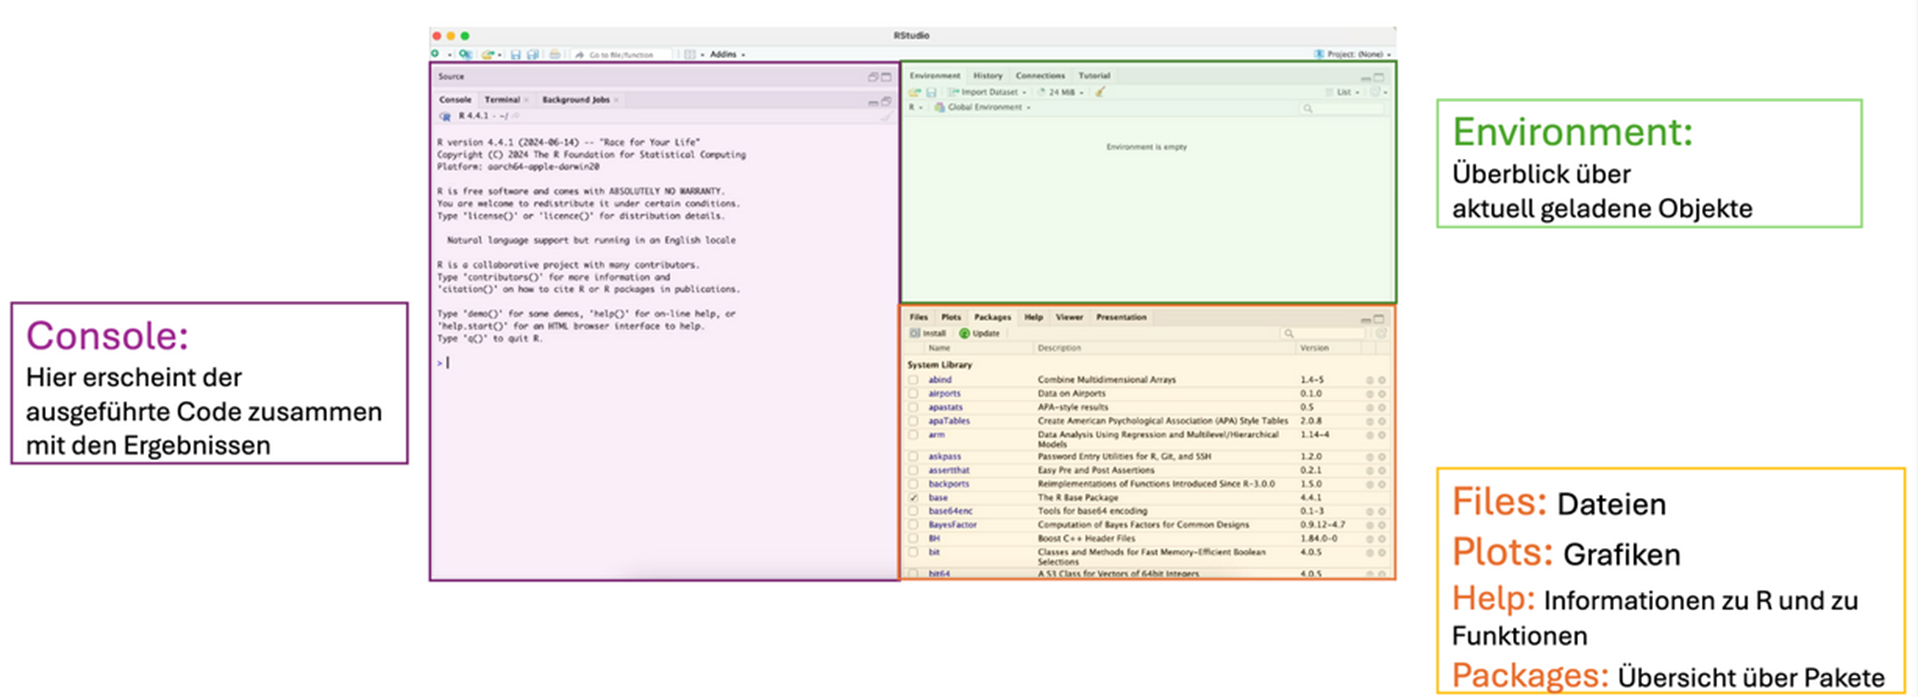
\includegraphics[keepaspectratio]{images/clipboard-2744485803.png}}




\end{document}
